\subsection{Evaluierung und Optimierung des Modells}
\label{sec:EvaluierungOptimierung}
In diesem Abschnitt werden zunächst Metriken festgelegt, mit denen die Performance von verschiedenen Modellen verglichen werden können.
Anschließend wird die Performance des bisherigen Modells anhand der Validierungsdaten evaluiert, indem untersucht wird, inwiefern die Vorhersagen des Modells von den konkreten Eingaben abhängen.
Zuletzt wird das Modell an verschiedenen Stellen verändert um zu erörtern, ob sich die Performance dadurch verbessern lässt.

Zunächst gilt es Metriken zu definieren, anhand derer verschiedene Modelle verglichen werden können.
Da Precision und Recall von der Perzentilgrenze abhängig sind, eignen sie sich nicht direkt.
Was sich hingegen eignet, ist die Precision-Recall-Kurve, da sie Precision und Recall über alle Perzentilgrenzen hinweg darstellt.
Zwei \acrshortpl{prc} verglichen werden, indem ermittelt wird, welche Kurve über der anderen liegt.
Jedoch erfolgt die Interpretation grafisch, obwohl der Vergleich von einzelnen Zahlenwerten oft einfacher ist.
Außerdem könnte bei verschiedenen Recall-Werten eine unterschiedliche Kurve die höhere Precision haben.
Eine Möglichkeit, eine komplette \acrshort{prc} in einem Zahlenwert zusammenzufassen besteht darin, die Fläche unter der Kurve zu berechnen.
Dieser Wert wird \acrfull{auprc} genannt.
Mit der \acrshort{auprc} kann die Performance eines Modells mit einer Zahl beschrieben werden und zwei Modelle können somit einfach verglichen werden.

Anhand der \acrshort{prc} und der \acrshort{auprc} soll nun zunächst das in den vorherigen Abschnitten implementierte Modell evaluiert werden.
Dabei soll auch eine der Kernfragen der vorliegenden Arbeit beantwortet werden.
Diese Kernfrage ist, ob sich die Standorte von mobilen Radarkontrollen anhand von historischen Daten und insbesondere derer der letzen 16 Tage vorhersagen lassen.
Besonders interessant ist hierbei, inwieweit die Vorhersagen konkret von den 16 Eingabeframes abhängt.
Wenn die Ausgabe praktisch unabhängig von den Eingabeframes wäre, würde eine rein statistische Auswertung des Datensatzes für die Vorhersagen genügen, wie z.\,B. die Identifizierung von Hotspots.
Um das Ausmaß der Abhängigkeit zu ermitteln bietet es sich an, die Zielframes zufällig zu vertauschen.
Somit kann überprüft werden, ob die Vorhersagen des Modells mit einem zufällig ausgewählten Raster genau so gut übereinstimmen wie mit dem Raster des tatsächlichen nächsten Tages.
Wenn dem so ist, sind die Vorhersagen weitestgehend unabhängig von den konkreten Eingabeframes.
Erzielt das Modell jedoch bessere Ergebnisse mit den wahren Zielframes, ist eine Abhängigkeit bestätigt.
Bevor die Überprüfung durchgeführt werden kann, sollte jedoch die Wahl des Validierungsdatensatzes angepasst werden.
In \autoref{sec:DatensatzLaden} wurde bisher definiert, dass sich die Sequenzen des Datensatzes beliebig überschneiden können, um eine größere Menge an Trainingsdaten zu erhalten.
Die erzeugten Sequenzen wurden dann zufällig dem Trainings- und Validierungsdatensatz zugewiesen.
Dies hat zur folge, dass sich die Sequenzen des Trainings- und Validierungsdatensatzes unter Umständen nur um zwei Frames unterscheiden - das erste und das letzte.
Dies hat auch zur Folge, dass die Zielframes des Validierungsdatensatzes im Trainingsdatensatz vorhanden sein können.
Somit hätte das Modell die Zielframes der Validierung schon gesehen, was die Evaluierung der Abhängigkeit verfälschen würde.
Um sicherzustellen dass dies nicht der Fall ist, werden die nach Anfangsdatum sortierten Sequenzen zunächst in Gruppen von je 34 Sequenzen unterteilt.
Da dieser Wert der doppelten Sequenzlänge inklusive der Zielframes entspricht, überschneiden sich die Gruppen nicht.
Als nächstes werden die Sequenzgruppen gemischt und zufällig in Trainings- und Validierungsdaten unterteilt.
Zuletzt werden die Trainings- und Validierungsdaten nochmals in sich gemischt.
Die resultierenden \acrshortpl{prc} sind in \autoref{fig:PRCValGetrennt} zu sehen.
Außerdem sind die \acrshort{auprc}-Werte der Kurven in der Legende aufgeführt.

\begin{figure}[h]
    \centering
    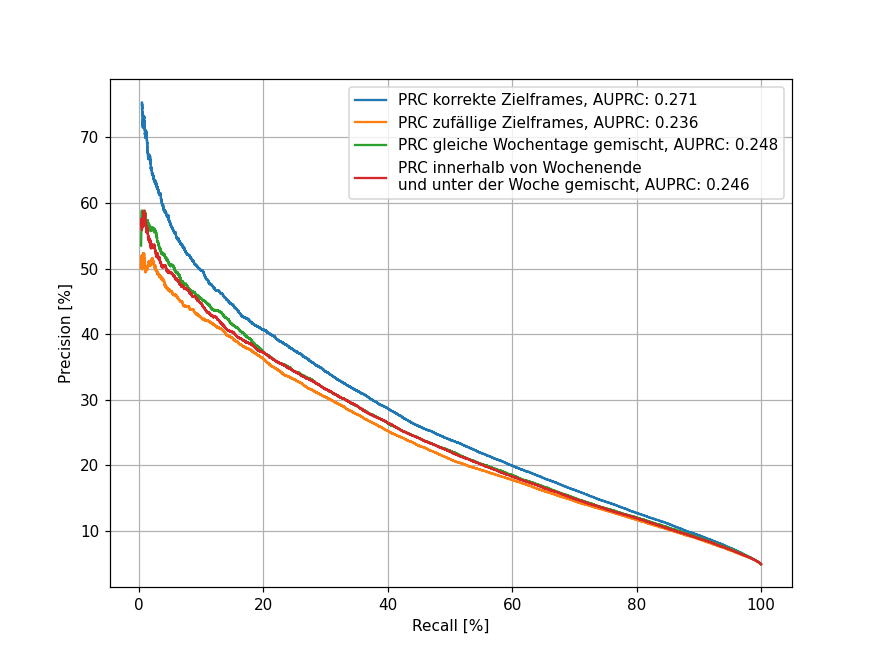
\includegraphics[width=1.0\textwidth,height=10cm,keepaspectratio=true]{content/images/PRCValGetrennt.png}
    \caption{\acrshortpl{prc} und \acrshort{auprc}-Werte mit wahren und gemischten Zielframes}
    \label{fig:PRCValGetrennt}
\end{figure}

Hierbei ist anzumerken, dass die \acrshortpl{prc} den Durchschnitt des gesamten Validierungsdatensatzes darstellen, und nicht wie in \autoref{fig:PredExGraphsPRC} nur eine einzelne Vorhersage.
Dadurch sind die Kurven weicher und regelmäßiger.
Es ist deutlich zu erkennen, dass die mit den zufälligen Zielframes erzeugte \acrshort{prc} (orange) am niedrigsten liegt und auch den geringsten \acrshort{auprc}-Wert von TODO aufweist.
Die \acrshort{prc} mit den korrekten Zielframes liegt hingegen höher, wie auch der \acrshort{auprc}-Wert von TODO.

